\section{Aufbau und Durchf"uhrung}
	\label{sec:durchfuehrung}

	Die Solarzelle wird gem"a"s Abb. \eqref{aufbau} angeschlossen.
	Die vier Solarzellen werden per Br"uckenstecker auf einer Rastersteckplatte mit einem  Amperemeter und einer Widerstandsdekade in Reihe geschaltet, parallel dazu ein Voltmeter.

	\begin{figure}[htbp]
		\centering
		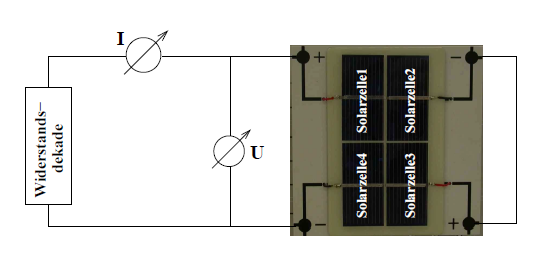
\includegraphics[width = 12cm]{img/aufbau.PNG}
		\caption{Schaltskizze zur Messung der I-U Kennlinie}
		\label{aufbau}
	\end{figure}

	"Uber der Solarzelle wird eine $\SI{120}{\watt}$ Lampe an einer h"ohenverstellbaren vorrichtung angebracht.
	Bei "uberbr"uckter Widerstandsdekade wird die h"ohe so eingestellt, dass der Kurzschlussstrom $I_K$ $\SI{30}{\milli\ampere}$, $\SI{50}{\milli\ampere}$, $\SI{75}{\milli\ampere}$ und $\SI{100}{\milli\ampere}$ betr"agt.
	Mit dem gr"o"sten Abstand wird die Messung begonnen.
	Nach unterbrechung des Stromkreises wird f"ur jede Messreihe die Leerlaufspannung $U_0$ gemessen.\\
	Um die Strom-Spannungs-Kennlinie der bei den einzelnen H"ohen zu bestimmen, wird nun die Br"ucke entfernt und die Widerstandsdekade von $\SI{1}{\ohm}$ bis $\SI{250}{\ohm}$ variier.
	Dabei wird nach jeder Messung die Leistung gemessen um m"oglichst zeitnah die Messpunkte um das Leistungsmaximum durchzuf"uhren.\\
	Aus den erhaltenen Daten wird nun der Wirkungsgrad bestimmt.